%% PODSTAWOWE USTAWIENIA DOKUMENTU
\documentclass[10pt, a4paper]{article}
\DeclareUnicodeCharacter{2003}{-}
%\usepackage[a4paper, lmargin=2.5cm, rmargin=2.5cm, hmargin=2.5cm, bmargin=2.5cm]{geometry}
\usepackage[a4paper,top=1cm,bottom=0.5cm,left=0.5cm,right=0.5cm]{geometry}
%\geometry{verbose,lmargin=2.5cm,rmargin=2.5cm}
\usepackage{enumerate}
% Symbole matematyczne
\usepackage{latexsym}
% Formatowanie czcionki
\usepackage[T1]{fontenc}
% Formatowanie polskich znaków
\usepackage{polski}
\usepackage[utf8]{inputenc}
% Akapit po sekcji
%\usepackage{indentfirst}
% Ustawienie nagłówków i stopek
\usepackage{fancyhdr}
% Liczba stron
\usepackage{lastpage}
% Kolumny
\usepackage{paracol}
% Czcionka latin modern
\usepackage{lmodern}
% Równania matematyczne
\usepackage{amsmath}
\usepackage{amsfonts}
\usepackage{amssymb}
\usepackage{amsthm}
% Wstawianie grafik
\usepackage{graphicx}
\usepackage[section]{placeins} % Ogarnięcie obrazków
\usepackage{float}
\usepackage{subcaption}
%\usepackage[outdir=./]{epstopdf}
\usepackage{grffile}

%% ODSTĘPY W WIERSZACH
\setlength{\parindent}{0.5cm}
\setlength{\parskip}{0.05cm}
\linespread{1}

%% SZARE TŁO TEKSTU
\usepackage[most]{tcolorbox}
\tcbset{
	frame code={}
	center title,
	left=0pt,
	right=0pt,
	top=0pt,
	bottom=0pt,
	colback=gray!30,
	colframe=white,
	width=\dimexpr\textwidth\relax,
	enlarge left by=0mm,
	boxsep=5pt,
	arc=0pt,outer arc=0pt,
}

% HIPERŁĄCZA SPISU TREŚCI
\usepackage{hyperref}
\hypersetup{
	colorlinks,
	citecolor=black,
	filecolor=black,
	linkcolor=black,
	urlcolor=black
}

\begin{document}
	\fancyhf{}	% Usunięcie domyślnego stylu numerowania
	
	% ********************** TYTUŁ ****************************
	\noindent\textsf{\begin{Large}Laboratorium Sterowania Adaptacyjnego \\\end{Large}
		Raport z ćwiczeń\textbf{ Ex4, Ex6}\\
		Szymon Kacperek, Adrianna Kręglewska, Adam Banaszczyk\\
		AiR, studia stacjonarne II stopnia,  specjalność SSiR, rok akademicki 2019/2020\\
		\rule{\columnwidth}{0.2pt}}
	
	\thispagestyle{empty}
	\pagestyle{fancy}
	\fancyhead{}
	\rhead{\thepage}
	\renewcommand{\headrulewidth}{0pt}%{}
	\setlength{\footskip}{1mm}
	
	%							*****************POCZĄTEK DOKUMENTU*****************
	\section{Model-Identification Adaptive Control (MIAC)}
	Celem projektu jest identyfikacja	 systemu za pomocą metody \textit{MIAC} z deterministyczną syntezą sterownika. Według założeń, \textit{MIAC} zapewnia asymptotyczną zbieżność błędu śledzenia do zera oraz czas ustalenia $T_{s1\%}=\alpha[s]$.
	
	Dla celów symulacji przyjęto następujące wartości parametrów:
	\begin{equation}
	T_a=0.005, \quad T_c=0.001, \quad  T_F=1.5T_a, \quad \hat{p}_0=[1 \quad 1], \quad \alpha=3.0,\quad lambda=0.999,\quad \rho = 0.1
	\end{equation}
	oraz postaci wymuszeń: \textbf{typu 1}: $y_r(t)=Y_r\sin(\omega_rt),\quad\dot{y}_r=Y_r\omega_r\cos(\omega_rt)$ oraz \textbf{typu 2}: $y_r(t)=Y_rrect(\omega_rt), \quad \dot{y}_r=0$.

\subsection{Wnioski}
Asymptotyczna zbieżność błędów śledzenia $e$ widoczna jest na rys. 3b, 3h i ulega pogorszeniu wraz ze wzrostem wariancji szumu białego (rys. 3d, 3f, 3j, 3l). Czas ustalenia $T_{s1\%}<\alpha$ (rys. 3h) został spełniony, lecz widoczna jest wrażliwość algorytmu na zakłócenia (rys. 3l), mogące doprowadzić do zmiany wartości tunelu ustalenia. Wraz ze wzrostem wariancji szumu białego, jakość odwzorowania trajektorii referencyjnej ulegała stopniowemu pogorszeniu (rys. 3f, rys. 3l), co ukazuje wrażliwość modelu na zakłócenia. Wpływ szumu białego na estymaty parametrów $\hat{p}$ obiektu ukazany jest na rysunku 1. 

Wykorzystanie sterownika ze stałym współczynnikiem $p$ nie spełniło założeń projektowych - uchyb nie zbiegał asymptotycznie do zera (rys. 2b, 2d). Wprowadzenie zmian (\textit{on-line}) parametru $w$ pozwoliło spełnić założenia projektowe. 

Wpływ czasu $T_a$ na przebiegi estymat parametrów widoczny jest na rys. 4a, 4b. Zwiększenie współczynnika $\rho$ oraz wpływ widoczny jest na rys 4c, 4d. 
	\subsection{Prezentacja wyników}	
	\begin{figure}[ht]\centering	
		a) 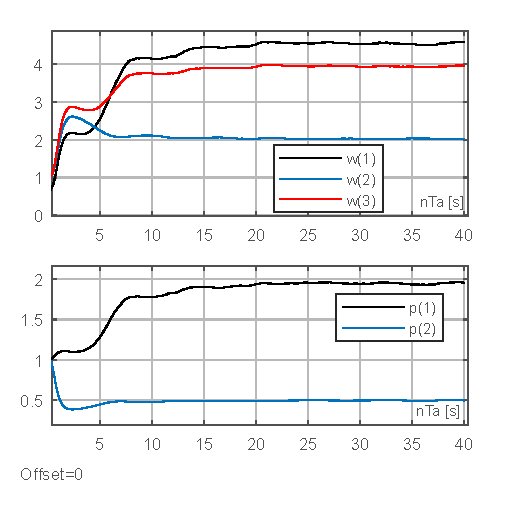
\includegraphics[width=0.31\columnwidth]{ACex4/ZADANIE3_1/figs/01Parametry_sigma001_sin} b)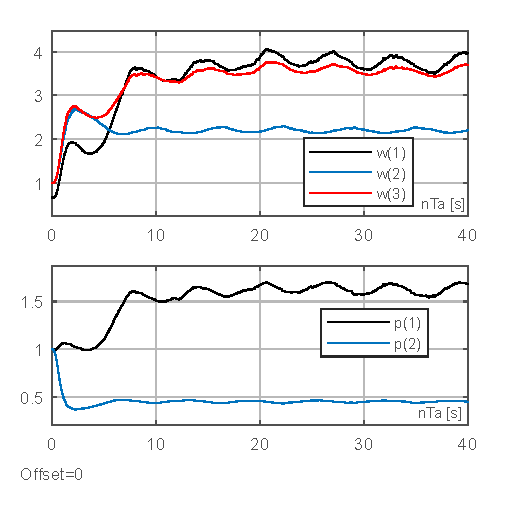
\includegraphics[width=0.31\columnwidth]{ACex4/ZADANIE3_1/figs/01Parametry_sigma01_sin} c)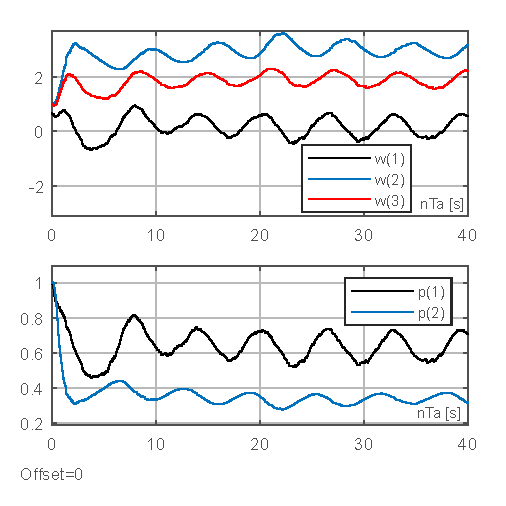
\includegraphics[width=0.31\columnwidth]{ACex4/ZADANIE3_1/figs/01Parametry_sigma10_sin}
		e) 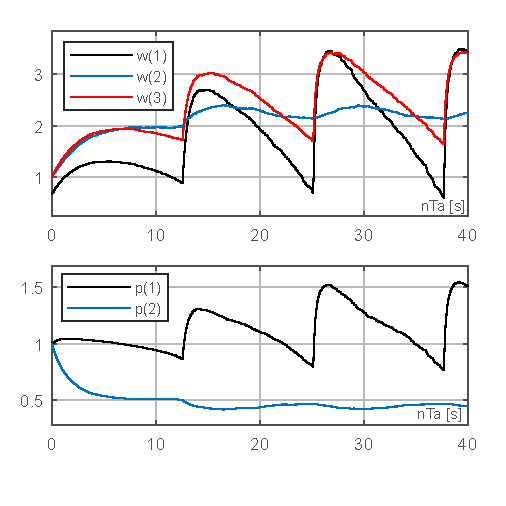
\includegraphics[width=0.31\columnwidth]{ACex4/ZADANIE3_1/figs/01Parametry_sigma001_rect} f)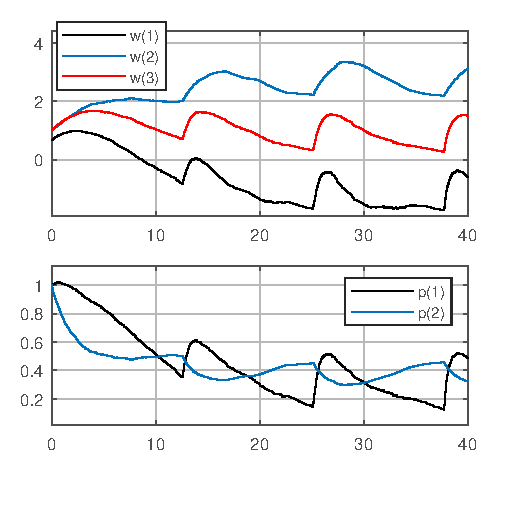
\includegraphics[width=0.31\columnwidth]{ACex4/ZADANIE3_1/figs/01Parametry_sigma01_rect} g)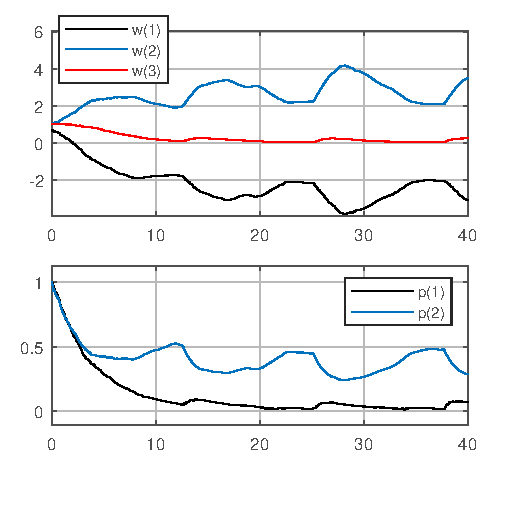
\includegraphics[width=0.31\columnwidth]{ACex4/ZADANIE3_1/figs/01Parametry_sigma10_rect}\caption{
			Wyniki symulacji bez sterownika dla zakłócenia szumem białym o wariancji (a, e) $\sigma^2_e=0.01$, (b, f) $\sigma^2_e=0.1$, (c, g)  $\sigma^2_e=1.0$ dla wymuszenia o wartościach współczynników $Y_r=1[rad/s]$,  $\omega_r=0.5[rad/s]$ typu 1 \textbf{(a-c)} oraz typu 2 \textbf{(d-f)}.}
	\end{figure}
	\begin{figure}[ht]\centering	
	a) 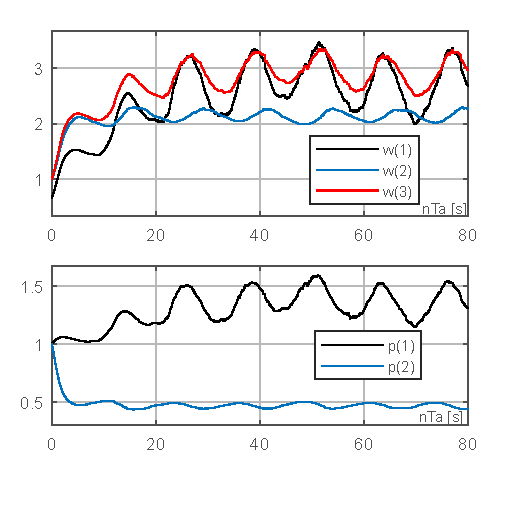
\includegraphics[width=0.22\columnwidth]{ACex4/ZADANIE3_2/figs/02Parametry_sigma001_sin} b)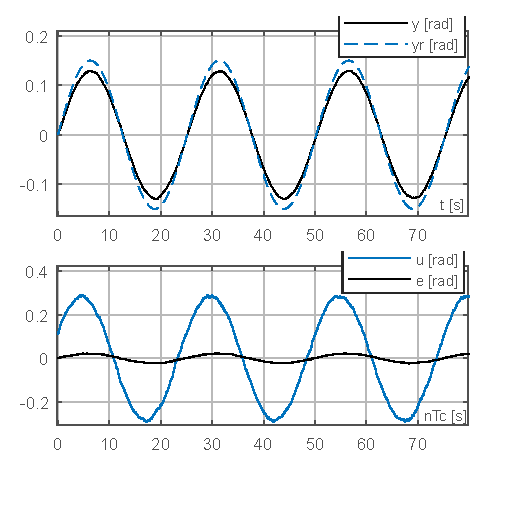
\includegraphics[width=0.22\columnwidth]{ACex4/ZADANIE3_2/figs/02Sygnaly_sigma001_sin} c)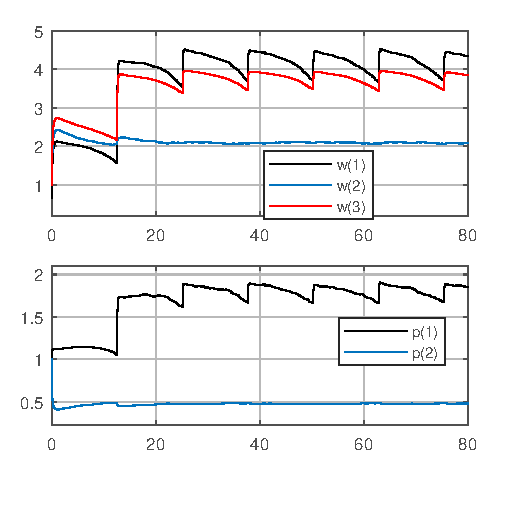
\includegraphics[width=0.22\columnwidth]{ACex4/ZADANIE3_2/figs/02Parametry_sigma001_rect}
	d) 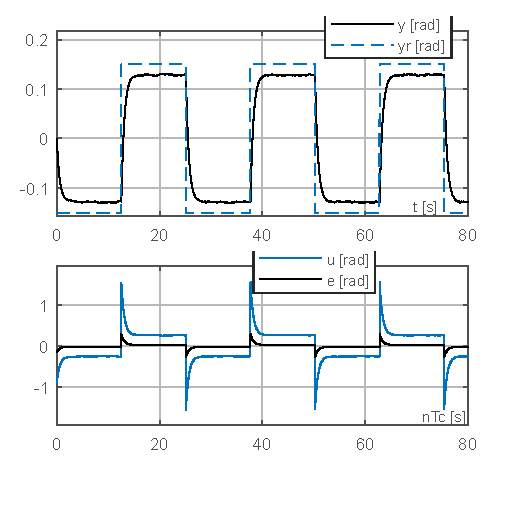
\includegraphics[width=0.22\columnwidth]{ACex4/ZADANIE3_2/figs/02Sygnaly_sigma001_rect} \caption{
		Wyniki symulacji z blokiem sterownika, o wartościach parametru $w=[5\quad1\quad1]$ dla zakłócenia szumem białym o wariancji 
		$\sigma^2_e=0.01$. Wymuszenia o wartościach współczynników 
		$Y_r=0.15[rad/s]$,  $\omega_r=0.25[rad/s]$ typu 1 \textbf{(a, b)} oraz typu 2 \textbf{(c, d)}.}
\end{figure}

	\begin{figure}[ht]\centering	
	a) 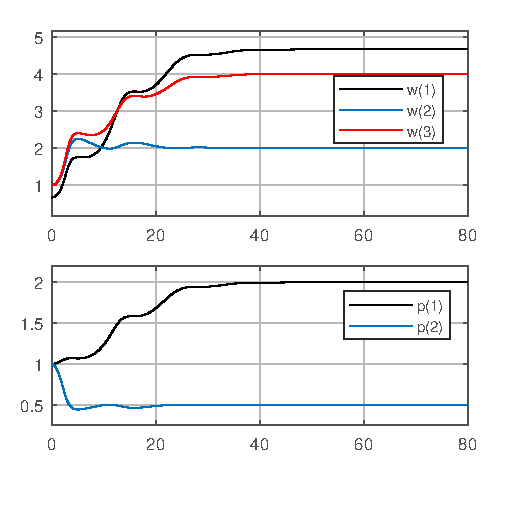
\includegraphics[width=0.22\columnwidth]{ACex4/ZADANIE3_3/figs/03Parametry_sigma00_sin} b)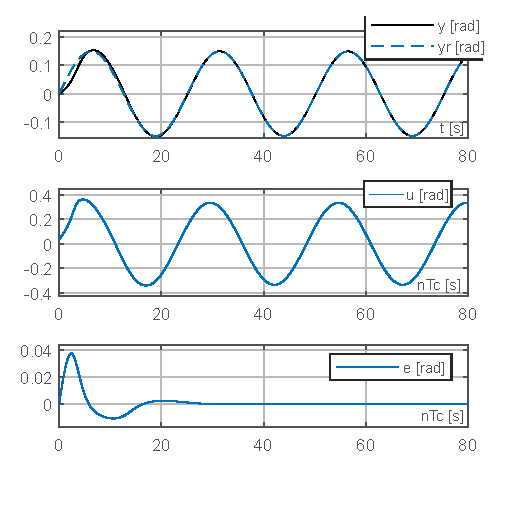
\includegraphics[width=0.22\columnwidth]{ACex4/ZADANIE3_3/figs/03Pozycje_sigma00_sin} c)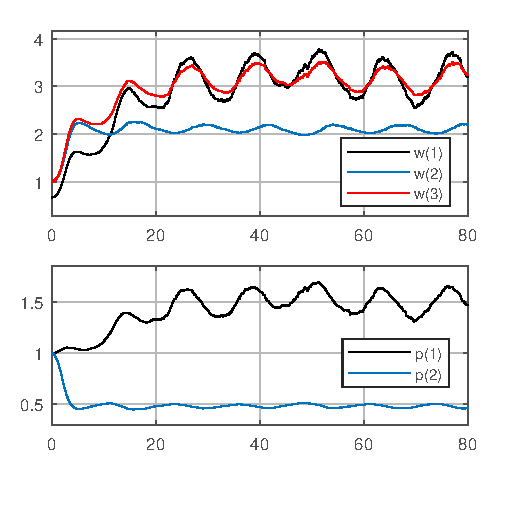
\includegraphics[width=0.22\columnwidth]{ACex4/ZADANIE3_3/figs/04Parametry_sigma001_sin}
	d) 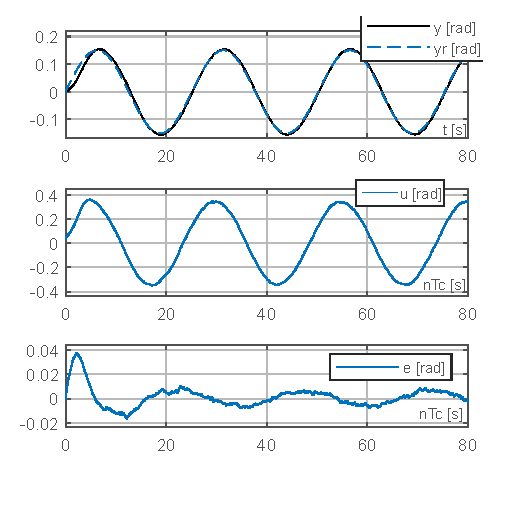
\includegraphics[width=0.22\columnwidth]{ACex4/ZADANIE3_3/figs/04Pozycje_sigma001_sin}\\
	e) 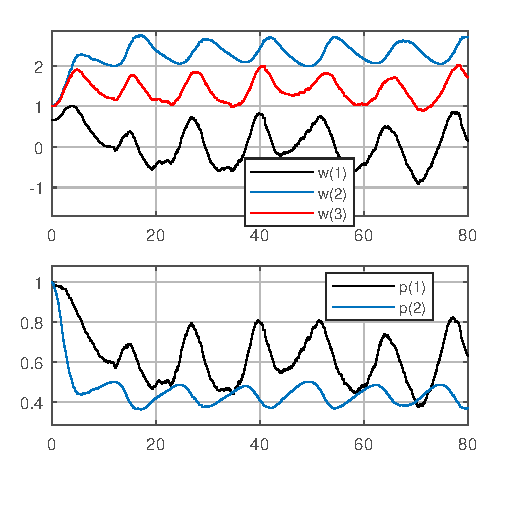
\includegraphics[width=0.22\columnwidth]{ACex4/ZADANIE3_3/figs/05Parametry_sigma01_sin} f)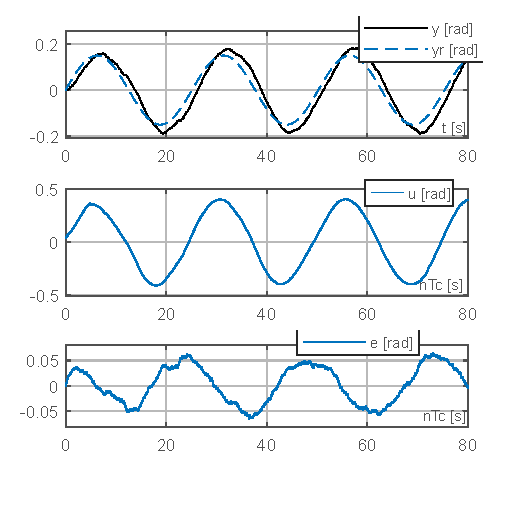
\includegraphics[width=0.22\columnwidth]{ACex4/ZADANIE3_3/figs/05Pozycje_sigma01_sin} g)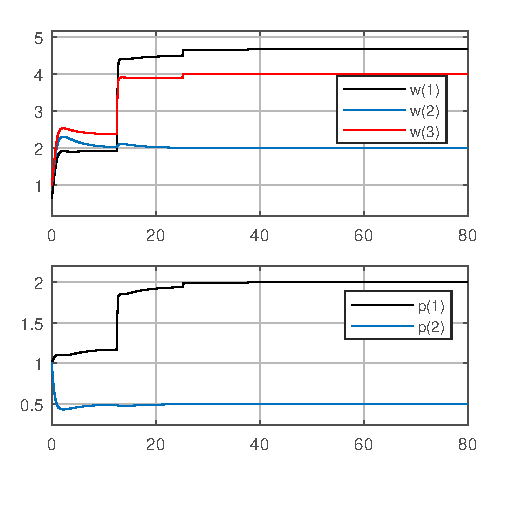
\includegraphics[width=0.22\columnwidth]{ACex4/ZADANIE3_3/figs/06Parametry_sigma00_rect}
	h) 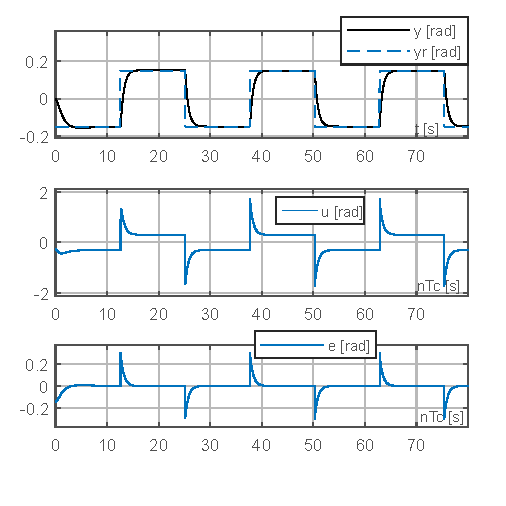
\includegraphics[width=0.22\columnwidth]{ACex4/ZADANIE3_3/figs/06Pozycje_sigma00_rect}\\
	i) 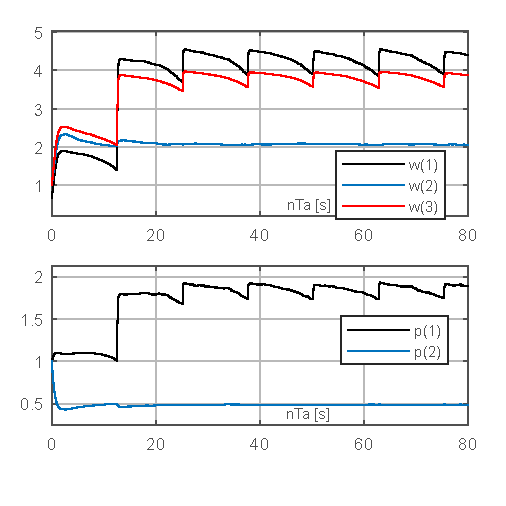
\includegraphics[width=0.22\columnwidth]{ACex4/ZADANIE3_3/figs/07Parametry_sigma001_rect} j)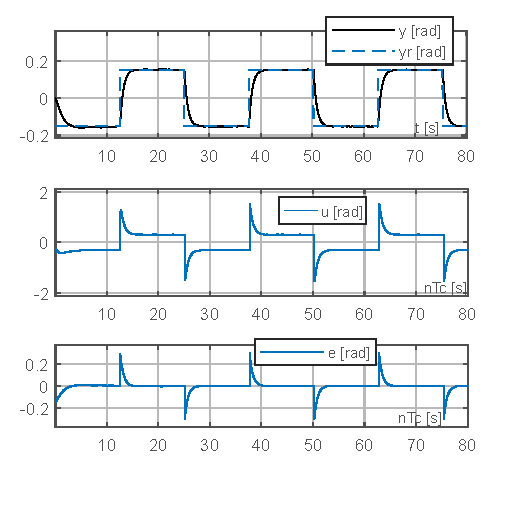
\includegraphics[width=0.22\columnwidth]{ACex4/ZADANIE3_3/figs/07Pozycje_sigma001_rect} k)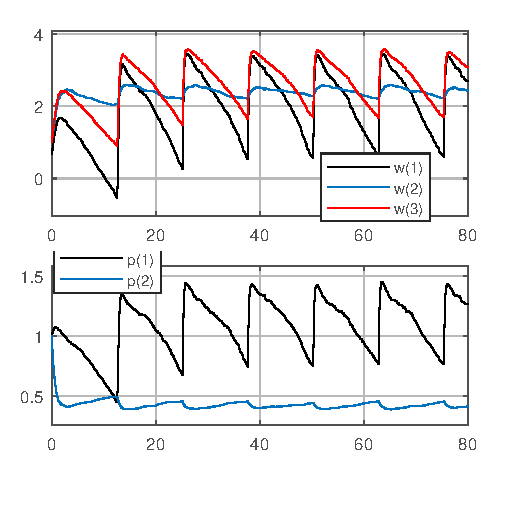
\includegraphics[width=0.22\columnwidth]{ACex4/ZADANIE3_3/figs/08Parametry_sigma01_rect}
	l) 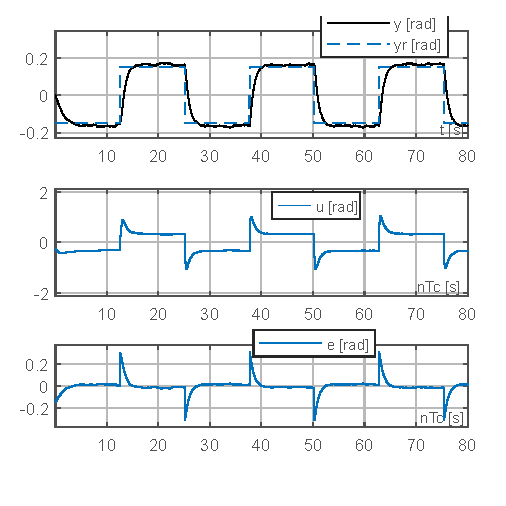
\includegraphics[width=0.22\columnwidth]{ACex4/ZADANIE3_3/figs/08Pozycje_sigma01_rect} \caption{
		Wymuszenia o wartościach współczynników $Y_r=0.15[rad/s]$,  $\omega_r=0.25[rad/s]$ typu 1 \textbf{(a-f)} oraz typu 2 \textbf{(g-l)}.
		Symulacja przeprowadzona z blokiem sterownika z adaptacyjną zmianą (\textit{on-line}) parametru $w$, dla zakłócenia szumem białym o wariancji
		(a, b, g, h) $\sigma^2_e=0.0$, (c, d, i, j) $\sigma^2_e=0.01$, (e, f, k, l)  $\sigma^2_e=0.1$.  Przebiegi współczynnika $w$, estymat parametrów $\hat{p}$ (a, c, e, g, i, k) oraz zadanej trajektorii referencyjnej $y_r$ oraz pozycji obiektu $y$, sygnału sterującego $u$ oraz błędu śledzenia $e$ (b, d, f, h, j, l).}
\end{figure}
	\begin{figure}[ht]\centering	
	a) \includegraphics[width=0.22\columnwidth]{ACex4/ZADANIE3_3/figs/09Parametry_Ta0002} b)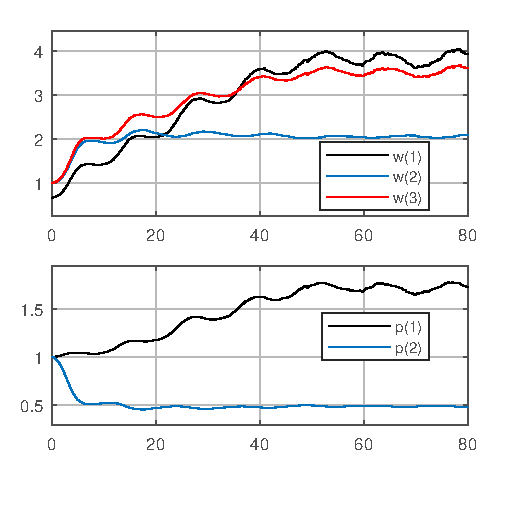
\includegraphics[width=0.22\columnwidth]{ACex4/ZADANIE3_3/figs/09Parametry_Ta0010} c)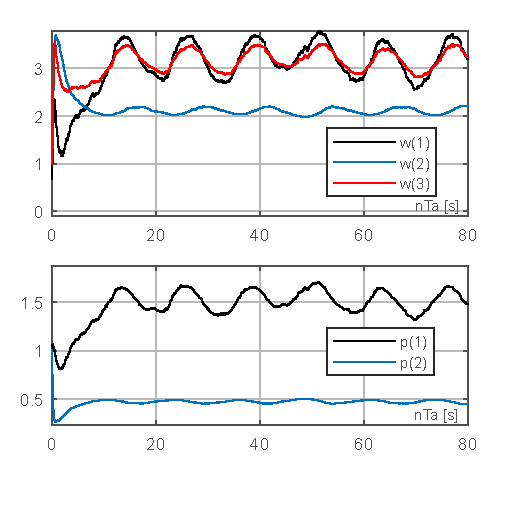
\includegraphics[width=0.22\columnwidth]{ACex4/ZADANIE3_3/figs/09Parametry_ro10}
	d) 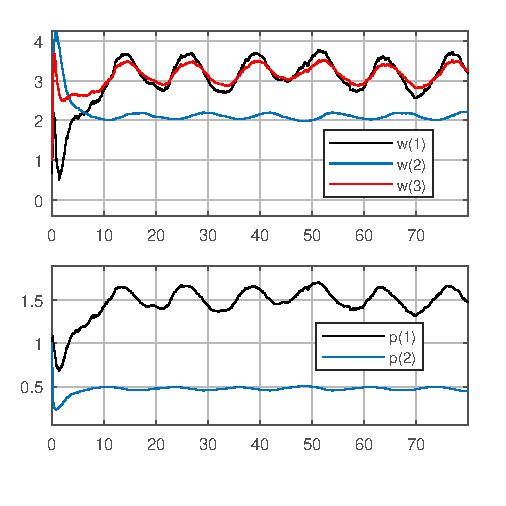
\includegraphics[width=0.22\columnwidth]{ACex4/ZADANIE3_3/figs/09Parametry_ro20} \caption{
	Wpływ parametrów $T_a$ a) 0.002, b) 0.01 oraz $\rho=$ c) 10, d) 20 na przebiegi estymat parametrów $\hat{p}$ oraz współczynnika $w$.}
\end{figure}

\section{Active/Adaptive Disturbance Rejection Control (ADRC)}

\subsection{Prezentacja wyników}
	\begin{figure}[ht]\centering	
	a) 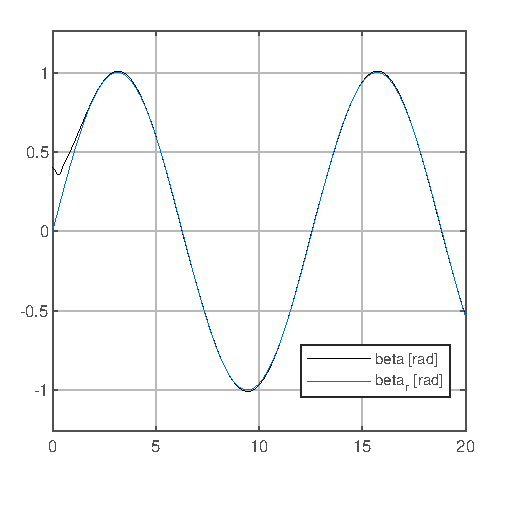
\includegraphics[width=0.22\columnwidth]{ACex6/figs/FIG1_a1_initial_tconst_sin_mi0.2/beta_betaref_initial_tconst_mi0.2} 
	b) 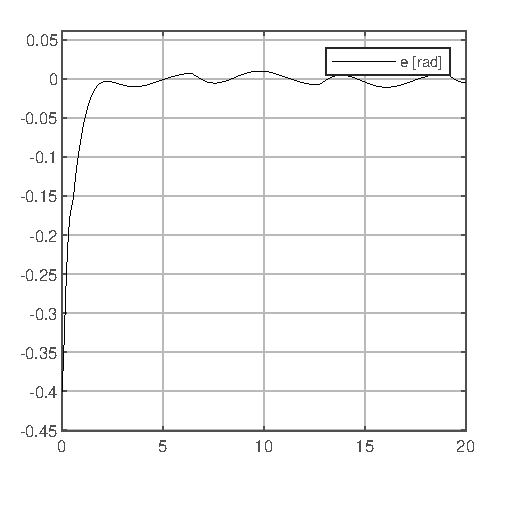
\includegraphics[width=0.22\columnwidth]{ACex6/figs/FIG1_a1_initial_tconst_sin_mi0.2/e_initial_tconst_mi0.2}
	c) 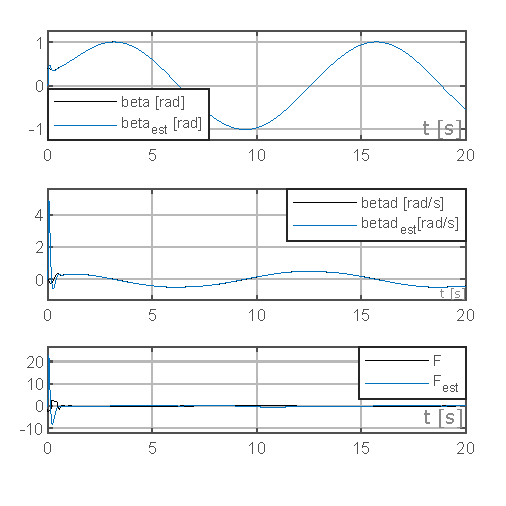
\includegraphics[width=0.22\columnwidth]{ACex6/figs/FIG1_a1_initial_tconst_sin_mi0.2/StateVar_initial_tconst_mi0.2}
	d) 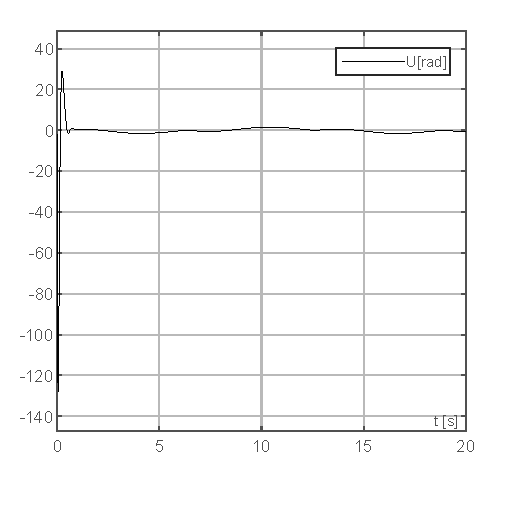
\includegraphics[width=0.22\columnwidth]{ACex6/figs/FIG1_a1_initial_tconst_sin_mi0.2/U_initial_tconst_mi0.2}\\
	e) 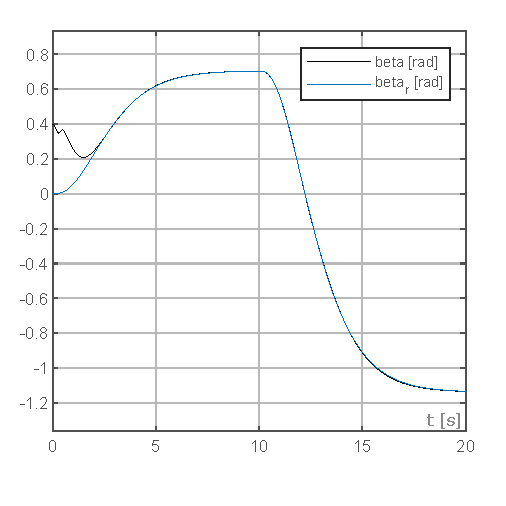
\includegraphics[width=0.22\columnwidth]{ACex6/figs/FIG1_a2_initial_tconst_rect_mi0.2/beta_betar_initial_tconst_rect_mi0.2} 
	f) 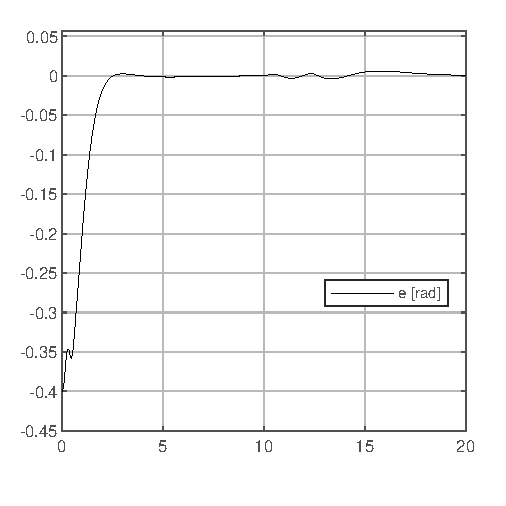
\includegraphics[width=0.22\columnwidth]{ACex6/figs/FIG1_a2_initial_tconst_rect_mi0.2/e_initial_tconst_rect_mi0.2}
	g) 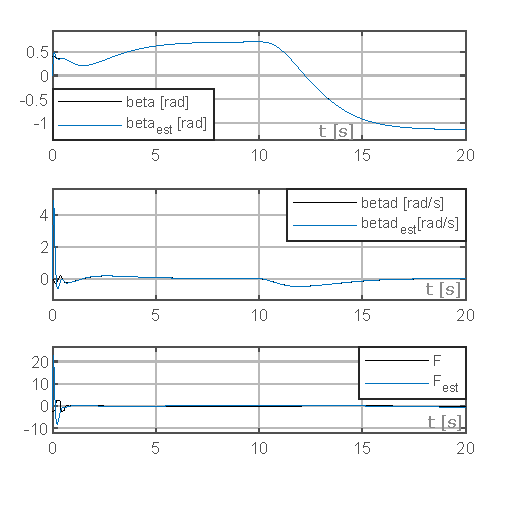
\includegraphics[width=0.22\columnwidth]{ACex6/figs/FIG1_a2_initial_tconst_rect_mi0.2/StateVar_initial_tconst_rect_mi0.2}
	h) 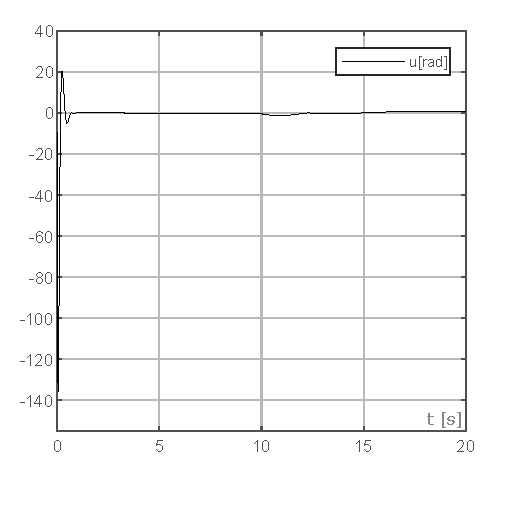
\includegraphics[width=0.22\columnwidth]{ACex6/figs/FIG1_a2_initial_tconst_rect_mi0.2/U_initial_tconst_rect_mi0.2}\\
	i) 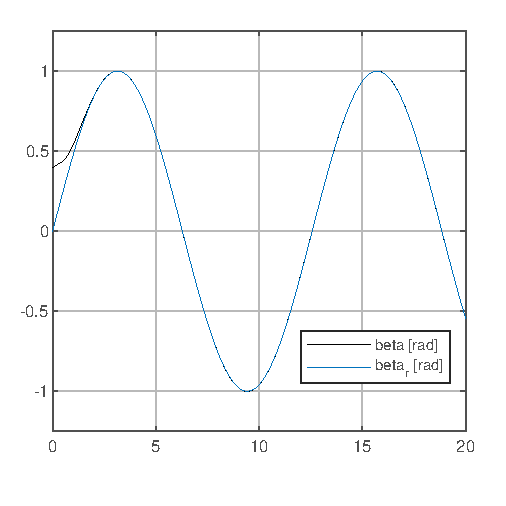
\includegraphics[width=0.22\columnwidth]{ACex6/figs/FIG1_b1_tconst_sin_mi0.03/beta_betar_tconst_sin_mi0.03}
	j) 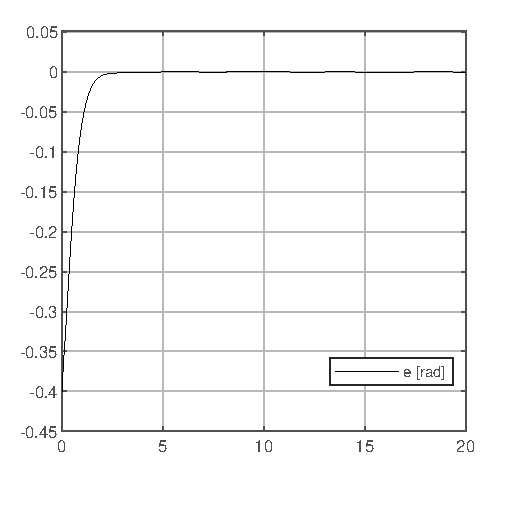
\includegraphics[width=0.22\columnwidth]{ACex6/figs/FIG1_b1_tconst_sin_mi0.03/e_tconst_sin_mi0.03}
	k) 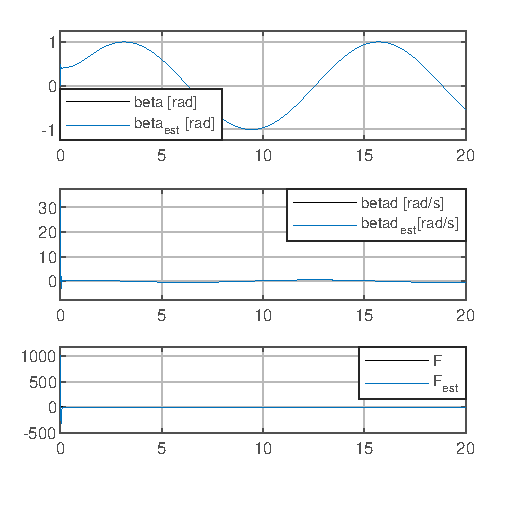
\includegraphics[width=0.22\columnwidth]{ACex6/figs/FIG1_b1_tconst_sin_mi0.03/StateVar_tconst_sin_mi0.03}
	l) 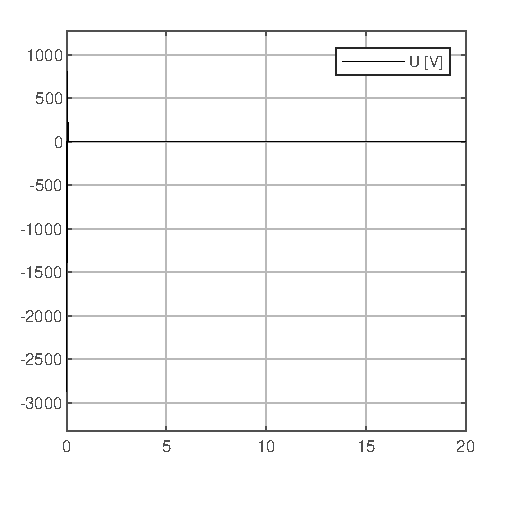
\includegraphics[width=0.22\columnwidth]{ACex6/figs/FIG1_b1_tconst_sin_mi0.03/U_tconst_sin_mi0.03}\\
	m) 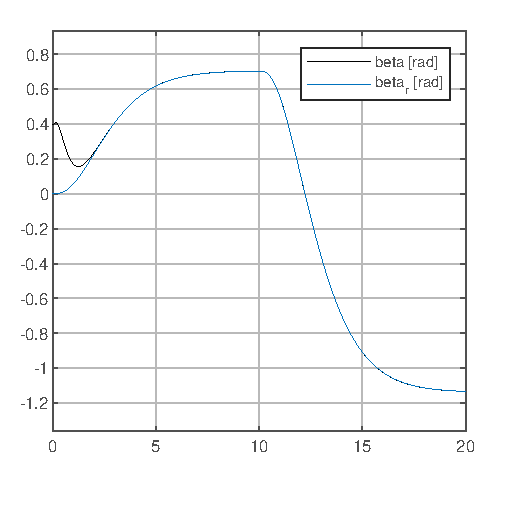
\includegraphics[width=0.22\columnwidth]{ACex6/figs/FIG1_b2_tconst_rect_mi0.03/beta_betar_tconst_rect_mi0.03}	
	n) 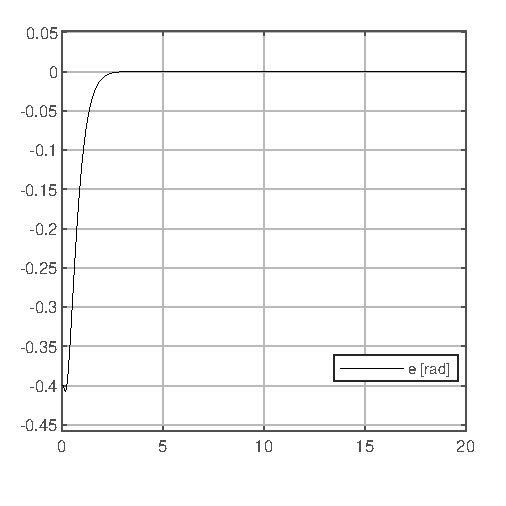
\includegraphics[width=0.22\columnwidth]{ACex6/figs/FIG1_b2_tconst_rect_mi0.03/e_tconst_rect_mi0.03}
	o) 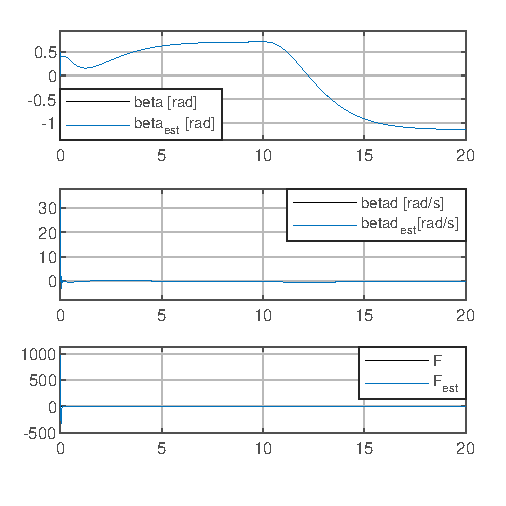
\includegraphics[width=0.22\columnwidth]{ACex6/figs/FIG1_b2_tconst_rect_mi0.03/StateVar_tconst_rect_mi0.03}
	u) 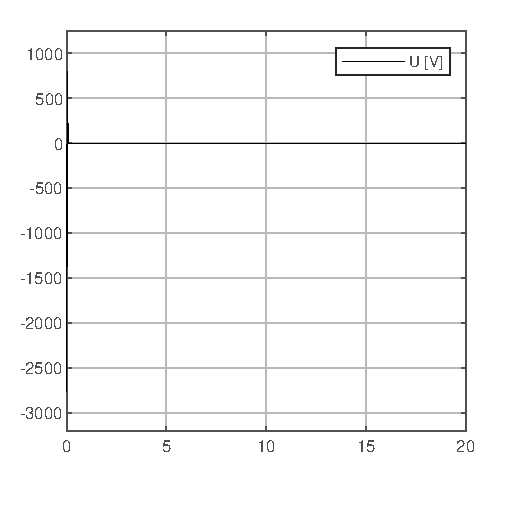
\includegraphics[width=0.22\columnwidth]{ACex6/figs/FIG1_b2_tconst_rect_mi0.03/U_tconst_rect_mi0.03}\\
	p) 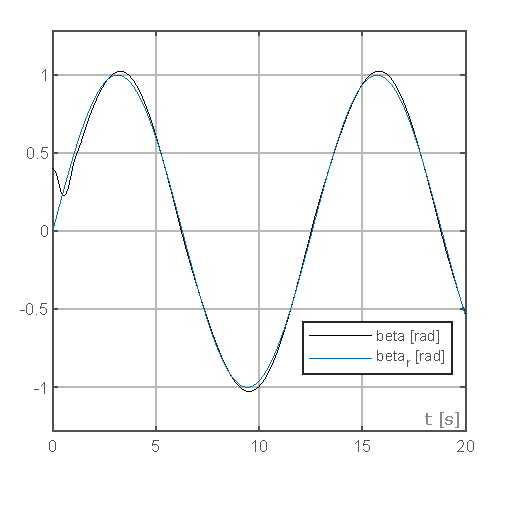
\includegraphics[width=0.22\columnwidth]{ACex6/figs/FIG1_c1_tconst_sin_mi0.5/beta_betar_tconst_sin_mi0.5}
	r) 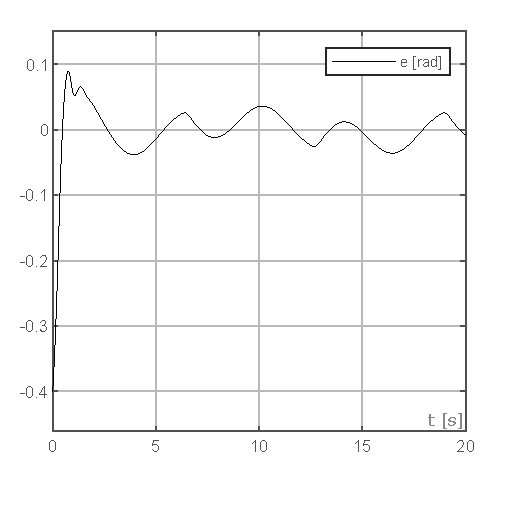
\includegraphics[width=0.22\columnwidth]{ACex6/figs/FIG1_c1_tconst_sin_mi0.5/e_tconst_sin_mi0.5}
	s) 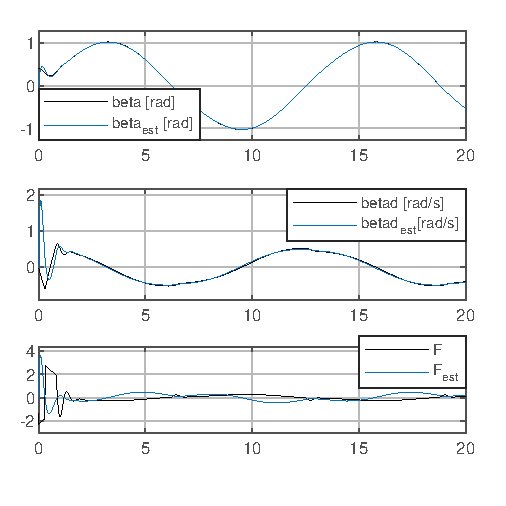
\includegraphics[width=0.22\columnwidth]{ACex6/figs/FIG1_c1_tconst_sin_mi0.5/StateVar_tconst_sin_mi0.5}
	t) 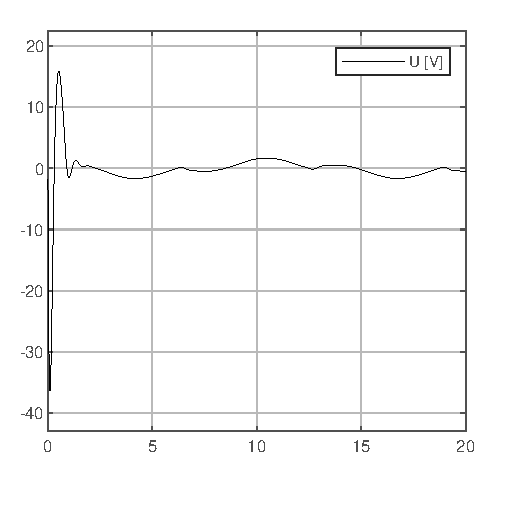
\includegraphics[width=0.22\columnwidth]{ACex6/figs/FIG1_c1_tconst_sin_mi0.5/U_tconst_sin_mi0.5}\\
	u) 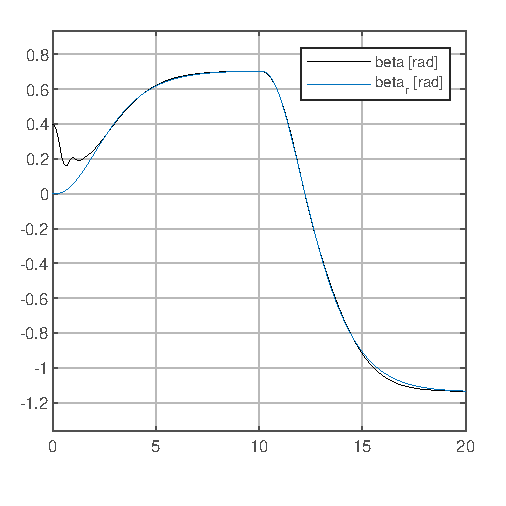
\includegraphics[width=0.22\columnwidth]{ACex6/figs/FIG1_c2_tconst_rect_mi0.5/beta_betar_rect_mi0.5}	
	w) 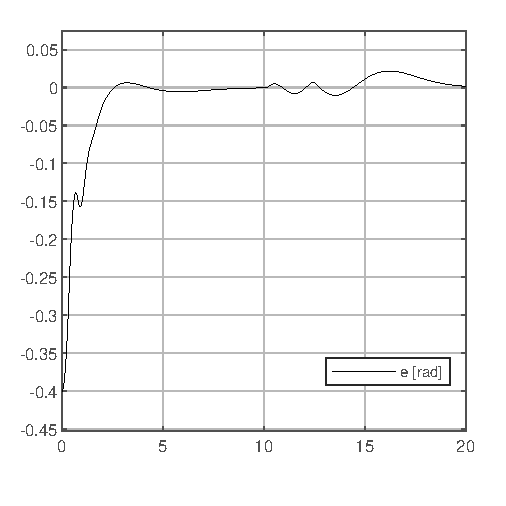
\includegraphics[width=0.22\columnwidth]{ACex6/figs/FIG1_c2_tconst_rect_mi0.5/e_tconst_rect_mi0.5}
	y) 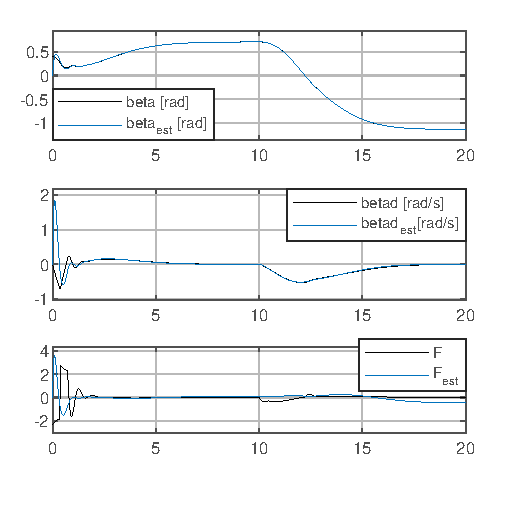
\includegraphics[width=0.22\columnwidth]{ACex6/figs/FIG1_c2_tconst_rect_mi0.5/StateVar_rect_mi0.5}	
	z) 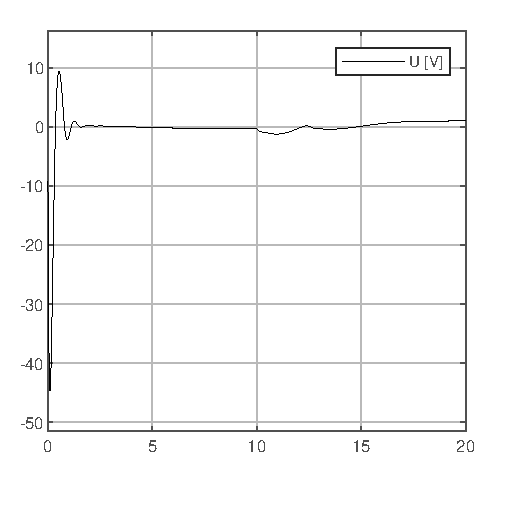
\includegraphics[width=0.22\columnwidth]{ACex6/figs/FIG1_c2_tconst_rect_mi0.5/U_rect_mi0.5}
		\caption{Warunki początkowe: mi = 0.2}
\end{figure}
	\begin{figure}[ht]\centering	
	a) \includegraphics[width=0.22\columnwidth]{ACex6/figs/FIG2_tconst_otwarcie_petli_adaptacji_(kompensacji)_sin_mi0.2/beta_betar_otwarciepetli_tconst_sin_mi0.2} 
	b) \includegraphics[width=0.22\columnwidth]{ACex6/figs/FIG2_tconst_otwarcie_petli_adaptacji_(kompensacji)_sin_mi0.2/e_otwarciepetli_tconst_sin_mi0.2}
	c) \includegraphics[width=0.22\columnwidth]{ACex6/figs/FIG2_tconst_otwarcie_petli_adaptacji_(kompensacji)_sin_mi0.2/StateVar_otwarciepetli_tconst_sin_mi0.2}
	d) \includegraphics[width=0.22\columnwidth]{ACex6/figs/FIG2_tconst_otwarcie_petli_adaptacji_(kompensacji)_sin_mi0.2/U_otwarciepetli_tconst_sin_mi0.2}\\
			\caption{otwarcie petli }
\end{figure}
	\begin{figure}[ht]\centering	
	a) \includegraphics[width=0.22\columnwidth]{ACex6/figs/FIG3_a_tconst_dON_sin_mi0.2/beta_betar_dON_tconst_mi0.2} 
	b) \includegraphics[width=0.22\columnwidth]{ACex6/figs/FIG3_a_tconst_dON_sin_mi0.2/e_dON_tconst_mi0.2}
	c) \includegraphics[width=0.22\columnwidth]{ACex6/figs/FIG3_a_tconst_dON_sin_mi0.2/StateVar_dON_tconst_mi0.2}
	d) \includegraphics[width=0.22\columnwidth]{ACex6/figs/FIG3_a_tconst_dON_sin_mi0.2/U_dON_tconst_mi0.2}\\
	e) \includegraphics[width=0.22\columnwidth]{ACex6/figs/FIG3_b_tconst_dON_otwartapetla_sin_mi0.2/beta_betar_dON_otwartapetla_tconst_mi0.2} 
	f) \includegraphics[width=0.22\columnwidth]{ACex6/figs/FIG3_b_tconst_dON_otwartapetla_sin_mi0.2/e_dON_otwartapetla_tconst_mi0.2}
	g) \includegraphics[width=0.22\columnwidth]{ACex6/figs/FIG3_b_tconst_dON_otwartapetla_sin_mi0.2/StateVar_dON_otwartapetla_tconst_mi0.2}
	h) \includegraphics[width=0.22\columnwidth]{ACex6/figs/FIG3_b_tconst_dON_otwartapetla_sin_mi0.2/U_dON_otwartapetla_tconst_mi0.2}\\
	\caption{A) mi = 0.2, dodanie zakłócenia zewnętrznego d; B) mi = 0.2, dodanie zakłócenia zewnętrznego d oraz otwarcie pętli kompensacji
	}
\end{figure}
	\begin{figure}[ht]\centering	
	a) \includegraphics[width=0.22\columnwidth]{ACex6/figs/FIG4_a_tdescrete_sin_Ta0.01/beta_betar_tdescrete_sin_Ta0.01} 
	b) \includegraphics[width=0.22\columnwidth]{ACex6/figs/FIG4_a_tdescrete_sin_Ta0.01/e_tdescrete_sin_Ta0.01}
	c) \includegraphics[width=0.22\columnwidth]{ACex6/figs/FIG4_a_tdescrete_sin_Ta0.01/StateVar_tdescrete_sin_Ta0.01} 
	d) \includegraphics[width=0.22\columnwidth]{ACex6/figs/FIG4_a_tdescrete_sin_Ta0.01/U_tdescrete_sin_Ta0.01}
	e) \includegraphics[width=0.22\columnwidth]{ACex6/figs/FIG4_b_tdescrete_sin_Ta0.04/beta_betar_tdescrete_sin_Ta0.04} 
	f) \includegraphics[width=0.22\columnwidth]{ACex6/figs/FIG4_b_tdescrete_sin_Ta0.04/e_tdescrete_sin_Ta0.04}
	g) \includegraphics[width=0.22\columnwidth]{ACex6/figs/FIG4_b_tdescrete_sin_Ta0.04/StateVar_tdescrete_sin_Ta0.04} 
	h) \includegraphics[width=0.22\columnwidth]{ACex6/figs/FIG4_b_tdescrete_sin_Ta0.04/U_tdescrete_sin_Ta0.04}
	\caption{Fig4: A) discrete Ta = 0.01 mi = 0.1 B) discrete Ta = 0.04 mi = 0.1}
\end{figure}
\end{document}
